High school math teaches us three things about algebra: first, that it is about meaingless symbols
like $x$ and $y$.\marginnote{
  \vspace{-0pt}
  \begin{center}
    \hspace{-10pt}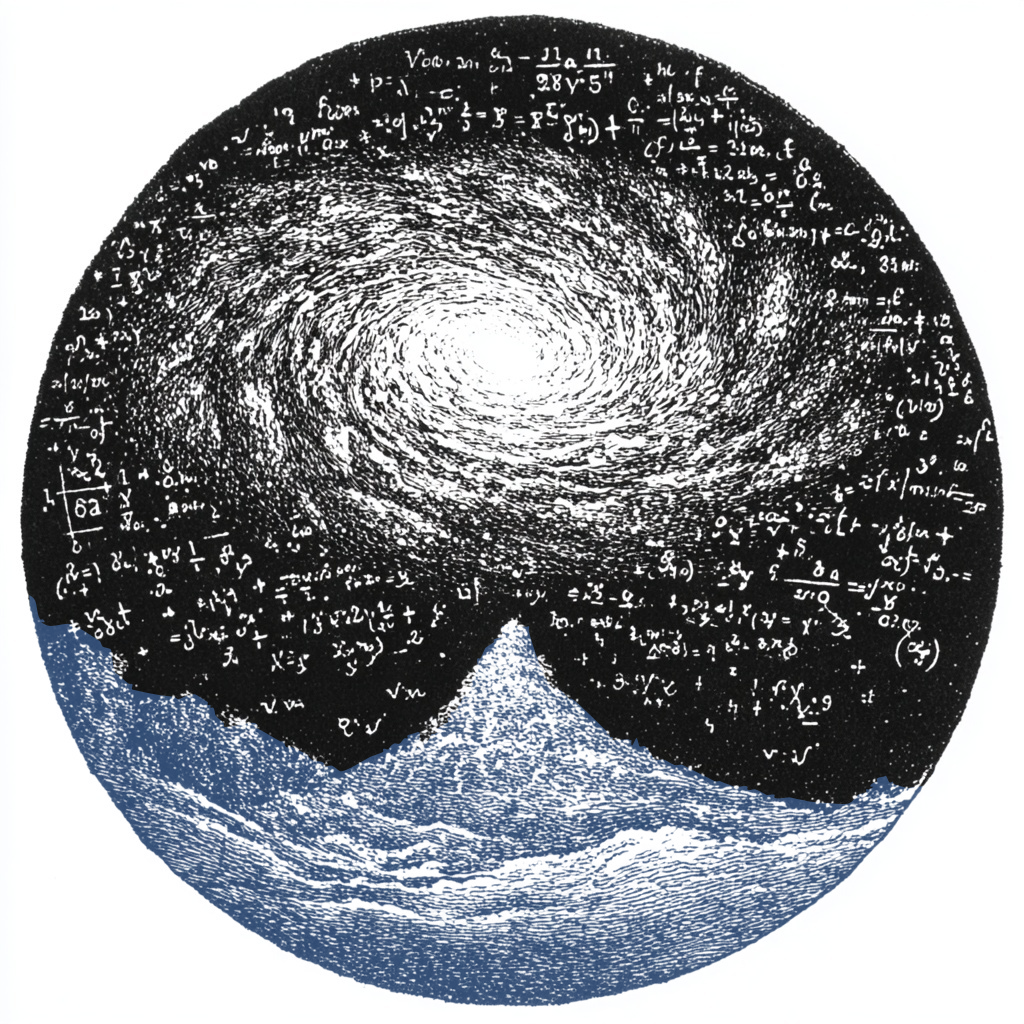
\includegraphics[width=1\linewidth]{img/algebra}
  \end{center}  \vspace{-5pt}
  \emph{The immortal truths of high school math.
  } \vspace{-10pt}
}
This is not so far from the truth, in quantum programming at least; we
call our meaningless symbols generators $\mathcal{G}$ and
use them to form our expressions. To construct an algebra with given
set of symbols \texttt{gens}, we invoke the global algebra variable \texttt{\$alg} and
equate it to \texttt{<gens|>}. The simplest thing we can create is
\begin{minted}
     [
frame=lines,
framesep=2mm,
baselinestretch=1.2,
bgcolor=AliceBlue,
fontsize=\footnotesize,
linenos
]{slurm}
    *> $alg = <X|>
  \end{minted}
namely the algebra generated by a single symbol $X$. This consists of
all products and linear combinations of $X$ with itself, i.e. the set
of complex polynomials in $X$, often called
$\mathbb{C}[X, X^*]$. We can
check that it simplifies as expected:
\begin{minted}
     [
frame=lines,
framesep=2mm,
baselinestretch=1.2,
bgcolor=AliceBlue,
fontsize=\footnotesize,
linenos
]{slurm}
    *> (X - 1)**2 - (X + 1)**2
    -4*X
  \end{minted}
% We can do basic high school algebra, for instance by setting $X = 1$:
% \begin{minted}{slurm}
%     *> X = 1
%     *> (X - 1)**2
%     0
%   \end{minted}
% This assignment renders all symbolic expressions in \texttt{X}
% numerical, so use with care!
  We can do straightup high school algebra as well:
  \begin{minted}
       [
frame=lines,
framesep=2mm,
baselinestretch=1.2,
bgcolor=AliceBlue,
fontsize=\footnotesize,
linenos
]{slurm}
    *> def quad(a, b, c):
    ...    delta = sqrt(b**2 - 4*a*c)
    ...    return [(-b+delta)/(2*a), (-b-delta)/(2*a)]
    *> x = quad(1, 4, 4)[0]
    *> x**2 + 4*x + 4
    0
  \end{minted}
The quadratic formula works! Now, back to our main programming.
  
The second thing we learn is that algebra is about solving equations. Once
again, this turns out to be fairly accurate, since the second ingredient in the
definition of an algebra is a set of \emph{relations} $\mathcal{R}$,
which are equations the generators satisfy. We use the constructor
\texttt{<gens|rels>}, where \texttt{rels} are either equations or
shorthands, e.g.
\begin{minted}   [
frame=lines,
framesep=2mm,
baselinestretch=1.2,
bgcolor=AliceBlue,
fontsize=\footnotesize,
linenos
]{slurm}
    *> $alg = <Y, Z | comm>
  \end{minted} 
which consists of all products and linear combinations of
\emph{commuting} $Y$ and $Z$, i.e. the polynomial ring
$\mathbb{C}[Y,Y^*,
Z, Z^*]$. Accordingly, we have identities like
\begin{minted}   [
frame=lines,
framesep=2mm,
baselinestretch=1.2,
bgcolor=AliceBlue,
fontsize=\footnotesize,
linenos
]{slurm}
    *> (Y - Z)**2 - (Y + Z)**2
    -4*Y*Z
  \end{minted}
as expected. So, if you want to play around with multivariate polynomials
(not exactly high school algebra) you can use \texttt{yaw} as well.
  
Nothing so far has the special structure needed to do quantum
computing. Loosely speaking, we want each generator $X$ to satisfy a
polynomial relation of the form $p(X, X^*) = 0$ with a bounded
solution set when restricted to $\mathbb{C}$. A simple example is the
algebra generated by a single unitary:
\begin{minted}
     [
frame=lines,
framesep=2mm,
baselinestretch=1.2,
bgcolor=AliceBlue,
fontsize=\footnotesize,
linenos
]{slurm}
    *> $alg = <U | unit>
    *> U*U.d
    I
  \end{minted}
where \texttt{U.d} stands for $U^*$.
A unitary $U$ satisfies the polynomial relation $p(U,U^*) = UU^*-  I =
0$,
and when interpreted over $\mathbb{C}$, the solutions are phases on
the unit circle, $\mathbb{S}^1 = \{e^{i\theta} : \theta\in
[0,2\pi)\}$, which is a manifestly bounded set.
The result can be viewed\sidenote{By something called \emph{Gelfand
    transform}, see Exercise 1.3.} as the C${}^*$-algebra of continuous
functions on the unit circle, $\mathcal{A}\cong C^0[\mathbb{S}^1]$.
In contrast, a single Hermitian operator satisfies a relation
$p(H, H^*) = H - H^* = 0$, which is solved by all real numbers:
\begin{minted}
     [
frame=lines,
framesep=2mm,
baselinestretch=1.2,
bgcolor=AliceBlue,
fontsize=\footnotesize,
linenos
]{slurm}
    *> $alg = <H | herm>
    *> H - H.d
    0
  \end{minted}
Since $\mathbb{R}$ is unbounded, the corresponding algebra
$\mathbb{C}[H]$ is \emph{not} C${}^*$, but rather a
polynomial ring over $\mathbb{C}$ with (formally) real variable.
% Equivalently, we can view it as the algebra of complex functions on
% the real line, $C^0[\mathbb{R}]$.

We could spend time constructing further examples of
infinite-dimensional C${}^*$-algebras, and indeed, these are relevant
to \emph{continuous variable} quantum computing, but we will defer their
treatment to a later tutorial.
Our focus will be on \emph{discrete variable} systems which have a
finite number of dimensions. In this case, we require only a finite
number of possible monomials built from generators. So, given two
generators $X$ and $Z$, the infinite list
\[
  X, X^2, \ldots, X^*, (X^*)^2, \ldots, Z, Z^2, \ldots, Z^*, (Z^*)^2 \ldots, XZ, (XZ)^2, \ldots
\]
must collapse to a finite set. That requires each of $X$, $X^*$, $Z$, $Z^*$, $XZ$,
etc, to have a finite \emph{order}, that is, a finite index such that
raising to that index gives the identity:
\[
  X^{\text{ord}(X)} = Z^{\text{ord}(Z)} = (XZ)^{\text{ord}(XZ)} =
  \cdots = I.
\]
It's simplest to set $\text{ord}(X)=\text{ord}(Z)=d$ equal by fiat,
and to implement $\text{ord}(X^*)=\text{ord}(Z^*) = d$ by taking $X$ and $Z$ unitary.
Enforcing that $XZ$ has finite order is a little trickier; the usual
approach is to allow $X$ and $Z$ to commute
\emph{up to a phase} $\omega$. This implies
\[
  ZX = \omega XZ \quad \Longrightarrow \quad (ZX)^d = \omega^{d(d-1)/2} Z^d  X^d =
  \omega^{d(d-1)/2} I,
\]
by counting the number of times we need to pass an $X$ over a $Z$.
When $\omega$ is a $d$th root of unity and $d$ is odd, then
$\omega^{d(d-1)/2} = 1$ and hence $\text{ord}(XZ) = d$; if $d$ is
even, then $\omega^{d(d-1)} = 1$ and $\text{ord}(XZ) = 2d$, or
equivalently, $\text{ord}(iXZ) = d$. Either way, we can take $\omega =
e^{2\pi i/d}$.

This leads to the final construction of this section. As above, we use
\texttt{unit} to make our operators unitary, and we introduce
\texttt{pow(d)} for the relations $X^d = Z^d = I$, and
\texttt{braid(w)} for $ZX = \omega XZ$:
\begin{minted}
     [
frame=lines,
framesep=2mm,
baselinestretch=1.2,
bgcolor=AliceBlue,
fontsize=\footnotesize,
linenos
]{slurm}
    *> $alg = <X, Z | unit, pow(d), braid(w)>
    *> X**d
    I
  \end{minted}
  This is the algebra of a \emph{qudit}, also known as the \emph{generalized
  Clifford algebra}. It has dimension $d^2$, since its elements are of
the form
\[
 A = \sum_{a,b=0}^{d-1} c_{ab} X^a Z^b.
\]
A special case is the trusty old Pauli algebra, $d = 2$, with relations
\[
  |X|^2 = X^2 = |Z|^2 = Z^2 = I, \quad XZ = -ZX.
\]
A phase $\omega = -1$ means $X$ and
$Z$ anticommute, which we also write
\begin{minted}   [
frame=lines,
framesep=2mm,
baselinestretch=1.2,
bgcolor=AliceBlue,
fontsize=\footnotesize,
linenos
]{slurm}
    *> $alg = <X, Z | unit, pow(2), anti>
  \end{minted}
To make life easier, \texttt{yaw} offers the shortcuts
\texttt{qudit(d)} and \texttt{qubit()} so you don't have to type
everything out
when defining algebras.

The third thing we learn in high school? That algebra has no application in
real life. Unlike the first two observations, this couldn't be
more wrong. Our thesis is that algebra is the foundation of quantum
mechanics; reality is quantum-mechanical; \emph{ipso facto}, reality
is based on algebra. Far from having no application,
algebra appears to ground \emph{reality itself}.
This might not make you rich or happy, but it will provide fodder
for undergraduate philosophy seminars, dinner parties, and obscure
programming paradigms.